\section{Results}
\label{sec:results}

We tested our methods on seventeen different $512\times 512$ gray scale images using six different algorithms:
\begin{enumerate}
	\item Sparse-coding with a DCT dictionary.
	\item Sparse-coding with a learned dictionary.
	\item Singular Value Decomposition.
	\item Regular diffusion with a $K_{\text{diamond}}$ kernel.
	\item Regular diffusion with a $K_{\text{gauss}}$ kernel.
	\item Directional diffusion with patches of size $32 \times 32$.
\end{enumerate}

 To test the performance of the algorithm, we consider a variety of masks:
\begin{enumerate}
	\item Nine different masks of randomly missing pixels distributed uniformly. These range from 10\% to 90\% missing pixels. This type of mask has many small missing regions.
	\item A mask represented by a sample of text. This type of mask has many medium-sized missing regions.
	\item A mask with large obfuscations such as squares and circles. This type of mask has a few large-sized missing regions.
\end{enumerate}

We have set up the experiments as follows: We take the original image $I$ and a mask $M$. We construct a damaged image $I_{\text{damaged}}$ based on $I$ but with the pixels indicated by the mask $M$ set to the fixed value 0. We run the relevant inpainting algorithms by providing it with both the damaged image and the mask. The algorithm will return us a recovered image $I^{\text{rec}}$, which we can compare with the original image $I$.

We compare the algorithms based on two criteria: the mean-squared error and the runtime of the algorithm. The mean-squared error is computed as the mean of the square of the difference in all pixel intensity values of the original image and the reconstructed image:
\begin{flalign*}
\text{MSE}(I, I^{\text{rec}}) = \frac{1}{512 \cdot 512} \sum_{i,j} (I_{i,j} - I^{\text{rec}}_{i,j})^2
\end{flalign*}


The mean-squared error of the algorithms for the randomly generated masks are displayed in figure \ref{fig:err_random} and the runtime is displayed in figure \ref{fig:runtime_random}.

The mean-squared error and runtime of the algorithms for the text mask is given in table \ref{tbl:err_text}.



\begin{table}
	\centering
	\begin{tabular}{|l|c|c|}
		\hline
		\textbf{Algorithm} & \textbf{MSE} & \textbf{Runtime} \\ \hline \hline
		Sparse-coding (DCT) & $0.0035 \pm 0.005$ & $50.7 \pm 3.2$ \\ \hline
		Sparse-coding (Learned) & $0.0024 \pm 0.009$ & $50.7 \pm 3.2$ \\ \hline
		Singular Value Decomposition & $0.0023 \pm 0.005$ & $50.7 \pm 3.2$ \\ \hline
		Diffusion ($K_{\text{diamond}}$) & $0.0020 \pm 0.03$ & $50.7 \pm 3.2$ \\ \hline
		Diffusion ($K_{\text{gauss}}$) & $0.0021 \pm 0.001$ & $50.7 \pm 3.2$ \\ \hline
		Directional Diffusion & $\mathbf{0.0018} \pm 0.002$ & $50.7 \pm 3.2$ \\ \hline
	\end{tabular}
	\caption{Mean-squared error and runtime (in seconds) across different algorithms for the text mask. The best result is highlighted in bold.}
	\label{tbl:err_text}
\end{table}

%\begin{figure*}
%	\begin{subfigure}[b]{0.48\textwidth}
%		\centering
%		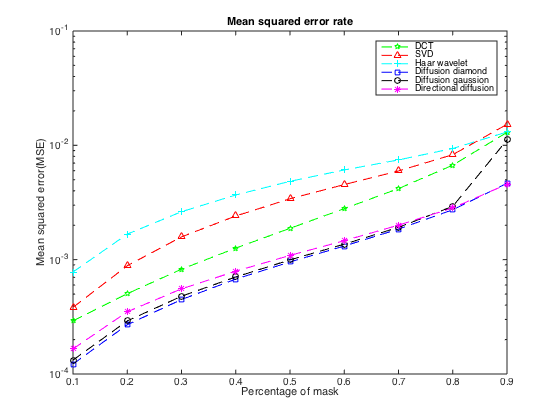
\includegraphics[trim=1.4cm 0.5cm 1.5cm 0.5cm, clip, width=0.9\textwidth]{figures/mse}
%		\caption{Mean square error }
%		\label{fig:mse}
%	\end{subfigure}
%	\begin{subfigure}[b]{0.48\textwidth}
%		\centering
%		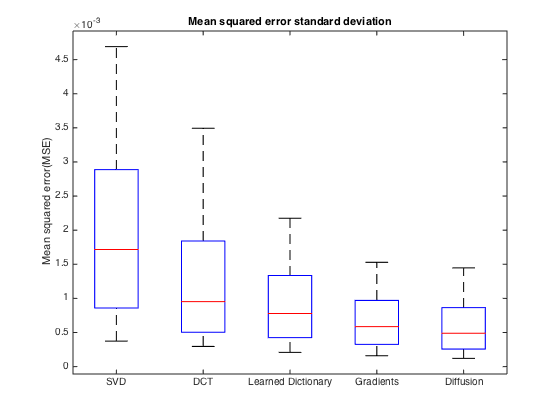
\includegraphics[trim=1.4cm 0.5cm 1.5cm 0.5cm, clip, width=0.9\textwidth]{figures/mse_std}
%		\caption{Standard deviation of mean squared error}
%		\label{fig:mse_std}	
%	\end{subfigure}
%\end{figure*}
